\documentclass[tikz,border=0pt]{standalone}
\usepackage{pgfplots}
\usepackage{xcolor}

\begin{document}

\begin{tikzpicture}
  [
    rec0/.style={shade,
                rectangle,
                minimum width=4mm,
                minimum height=1.5mm,
                inner sep=0pt,
                outer sep=0pt,
                top color=gray!60!white,
                bottom color=gray!30!white,
                draw=black, 
                very thin},
    rec16/.style={shade,
                rectangle,
                rotate=16,
                minimum width=4mm,
                minimum height=1.5mm,
                inner sep=0pt,
                outer sep=0pt,
                top color=gray!60!white,
                bottom color=gray!30!white,
                draw=black, 
                very thin},
    rec16r/.style={shade,
                rectangle,
                rotate=-16,
                minimum width=4mm,
                minimum height=1.5mm,
                inner sep=0pt,
                outer sep=0pt,
                top color=gray!60!white,
                bottom color=gray!30!white,
                draw=black, 
                very thin},
    rec45/.style={shade,
                rectangle,
                rotate=45,
                minimum width=10mm,
                minimum height=3.75mm,
                inner sep=0pt,
                outer sep=0pt,
                top color=gray!60!white,
                bottom color=gray!30!white,
                draw=black, 
                very thin}
  ]
% width is 8.64cm
\newcommand{\figwidth}{8.64cm}
\newcommand{\figheight}{5.33cm}

\draw[use as bounding box, white] (0,0) rectangle (\figwidth,\figheight);

% Setup
\begin{scope}[
    xshift=1.5cm,
    yshift=2.7cm
    ]
    \node[inner sep=0pt]  at (0,0)
        {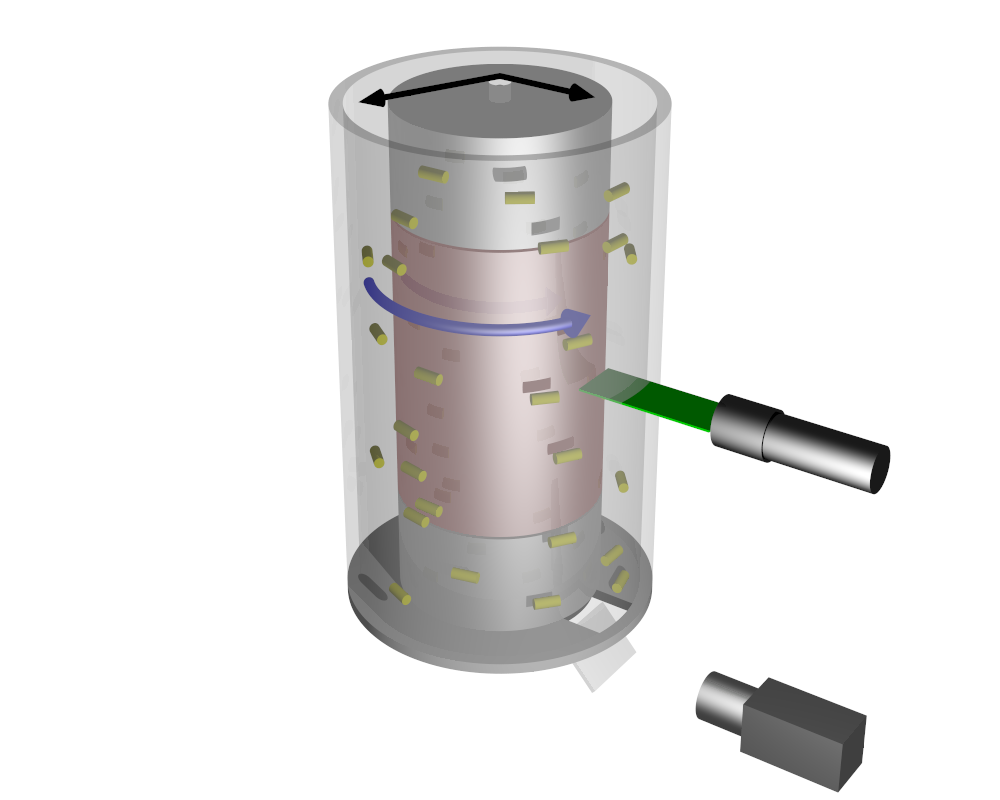
\includegraphics[
            height=\figheight,
            trim={5cm, 0.25cm, 3.8cm, 0}, 
            clip
        ]{t3csetup.png}};
\end{scope}

% Still image
\begin{scope}[
    xshift=6.41cm,
    yshift=1.39cm
    ]
    \node[inner sep=0pt]  at (0,0)
        {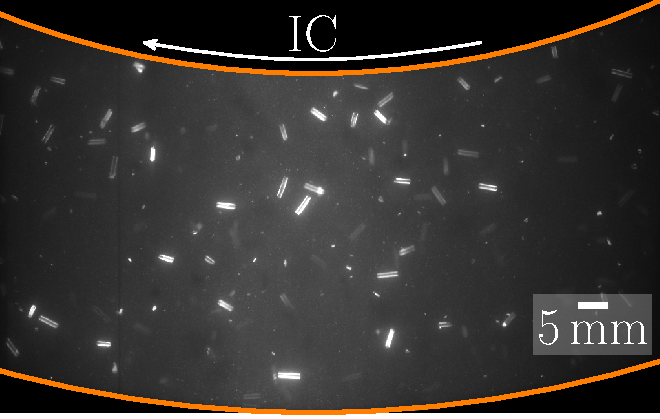
\includegraphics[
            width=4.4cm,
            %trim={5cm, 0.25cm, 3.8cm, 0}, 
            %clip
        ]{stillimage.pdf}};
\end{scope}

% Cylinder
\begin{scope}[
     xshift=6.37cm,
     yshift=9.8cm,
     scale=3.75,
     every node/.append style={transform shape},
    ]
    \clip (-0.487, -1.220) rectangle (0.502, -1.86);

    % Outer cylinder and water inside
    \draw[color=black, fill=white, thin] (0, 0) circle (1.851);

    % inner cylinder
    \draw[color=black, fill=gray!10, thin] (0, 0) circle (1.325);

    \draw[color=black, dashed, thick] (-0.487, -1.25) -- (-0.487, -1.79);
    \draw[color=black, dashed, thick] (0.502, -1.243) -- (0.502, -1.79);
    \draw[color=black, dashed, thick] (-0.487, -1.220) -- (0.502, -1.220);
    \node at (0.025, -1.275) {\scalebox{0.28}{IC}};

    % dashed center line
    \draw[color=red, thick, densely dotted] (0, 0) circle (1.588);

    % filled polygon
    \coordinate (L1) at (-0.487, -1.79);
    \coordinate (L2) at (-0.487, -1.233);
    \coordinate (L3) at (-0.360, -1.275);
    \fill[color=red, opacity=0.2] (L1) -- (L2) -- (L3) -- cycle;
    \coordinate (R1) at (0.502, -1.79);
    \coordinate (R2) at (0.502, -1.228);
    \coordinate (R3) at (0.375, -1.272);
    \fill[color=red, opacity=0.2] (R1) -- (R2) -- (R3) -- cycle;
 \end{scope}

% big fiber representation
\begin{scope}[
     xshift=6.42cm,
     yshift=5.6cm,
     scale=0.5
    ]
    \path (0, -3.50) coordinate[rec45];  
    \draw[color=black, densely dashed, thick] (-1.5, -5) -- (1.10, -2.4);
    \draw[color=red, thick] (-2, -3.5) -- (1.10, -3.5);
    \draw[color=blue] (-1.5, -3.5) arc (180:225:15mm);
    \node at (-1.70, -4.25) {\scalebox{1.5}{$\theta_p$}};
\end{scope}
    
    % labels
    \node at (0.20cm, 5.15cm) {(a)};
    \node at (4.20cm, 5.15cm) {(b)};
    \node[white] at (4.45cm, 2.35cm) {(c)};

    \node at (1.35, 3.4) {\Large$\omega_i$};
    \node at (1.7, 4.98) {\Large$r_i$};
    \node at (0.90, 5.0) {\Large$r_o$};

\end{tikzpicture}
\end{document}
